\documentclass{szzclass}
\usepackage[margin=3cm]{geometry}
\subject{SI1.2}
\code{BI-WSI-SI-18}
\topic{Analýza a správa požadavků (cíle, kategorizace, UML diagram případů užití, scénáře případů užití, UML diagram aktivit).}

\begin{document}

\section{Analýza a správa požadavků}
\subsection{Cíle}
\begin{itemize}
\item Vymezit hranice systému
\item Umožnit přesnější odhad pracnosti
\item Vyjasnit si zadání se zákazníkem
\item Zachytit omezení, která jsou na IS kladena
\end{itemize}

\subsection{Kategorizace základní}
\begin{itemize}
\item Funkční
\item Obecné (Nefunkční)
  \begin{itemize}
  \item Určují omezení kladená na systém
  \item Mají zásadní dopad na návrh architektury
  \item Určují dodržování standardů
  \end{itemize}
\end{itemize}

\subsection{FURPS}
\begin{description}
\item[F (functionality)] - funkčnost
\item[U (usability)] - použitelnost
\item[R (reliability)] - spolehlivost
\item[P (performace)] - výkon
\item[S (supportability)] – podporovatelnost / rozšiřitelnost
\end{description}

\subsection{Evidované informace}
\begin{itemize}
\item Název požadavku
\item Zkratka – usnadňuje odkazování na požadavek
\item Popis – nejdůležitější část
\item Typ (kategorie)
\item Priorita
\item Složitost
\end{itemize}

\subsection{Zdroje informací}
\begin{itemize}
\item Komunikace se zákazníkem
\item Model obchodních procesů
\item Zadávací dokumentace
\end{itemize}

\subsection{Splnění požadavků}
\begin{itemize}
\item vždy ověřitelné
\item jasné
\item priority
\end{itemize}


\section{Případy užití}
\begin{itemize}
\item Detailní specifikace funkčních požadavků.
\item Typicky se jednotlivé požadavky rozpadají na několik případů užití.
\item Skládá se z:
  \begin{itemize}
    \item Seznam účastníků
    \item Diagram případů užití
    \item Seznam případů užití (název, zkratka, popis, scénář, podmínky)
  \end{itemize}
\end{itemize}

\subsection{Využití}
\begin{itemize}
\item Základ pro tvorbu uživatelské příručky
\item Podklady k tvorbě akceptačních testů
\item Zpřesnění odhadů pracnosti
\item Zadání pro programátora
\end{itemize}

\subsection{Chyby}
\begin{itemize}
\item Diagram případů užití nemá znázorňovat tok událostí. (Od toho jsou jiné typy diagramů.)
\item Diagram případů užití nemá znázorňovat datové paměti.
\item Případ užití bez účstníků nemá žádný význam.
\item Případy užití nenaznačují komunikaci mezi aktéry.
\item Počet funkčních požadavků nemá být stejný jako počet případů užití.
\end{itemize}

\section{Modelování}
\subsection{Případy užití}
\begin{description}
\item[include] - Začlenění shodných částí scenaru
\item[extend] - Společná část nemusí být povinná
\end{description}

\subsection{Diagram aktivit}
\begin{itemize}
\item Ve skupině diagramů chování
\item Swimlines - Zóny zodpovědnosti
\item Objektový uzel - Zachycení stavu objektu
\end{itemize}

\begin{figure}[ht!]
\centering
\begin{minipage}{.5\textwidth}
\begin{itemize}
    \item Aktivita
    \item Odeslání události
    \item Přijetí události
    \item Časová událost
\end{itemize}
\end{minipage}%
\begin{minipage}{.5\textwidth}
\begin{itemize}
    \item Počáteční uzel
    \item Koncový uzel
    \item Rozhodnutí (větvění/spojení)
    \item Paralelní souběh (fork/join)
    \item Konec toku
\end{itemize}
\end{minipage}
\end{figure}

\begin{figure}[ht!]
\centering
\begin{minipage}{.5\textwidth}
  \centering
  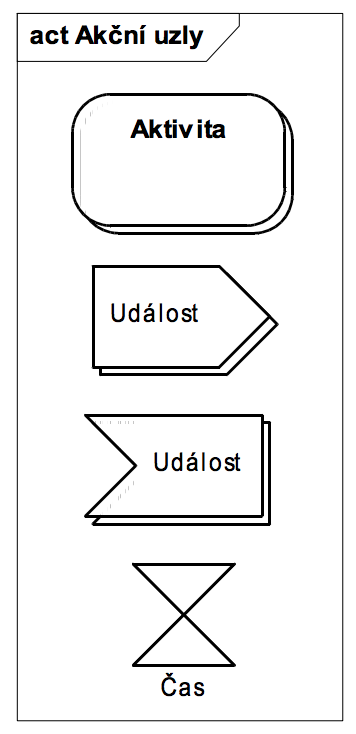
\includegraphics[width=.75\linewidth]{topics/bi-wsi-si-18/images/akcni-uzly.png}
  \caption{Akční uzly}
\end{minipage}%
\begin{minipage}{.5\textwidth}
  \centering
  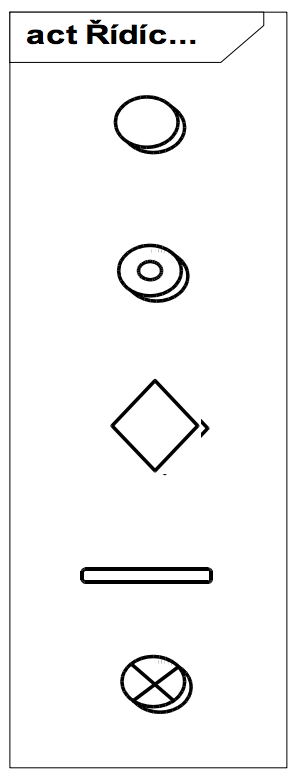
\includegraphics[width=.75\linewidth]{topics/bi-wsi-si-18/images/ridici-uzly.png}
  \caption{Řídící uzly}
\end{minipage}
\end{figure}

\begin{figure}[ht!]
\centering
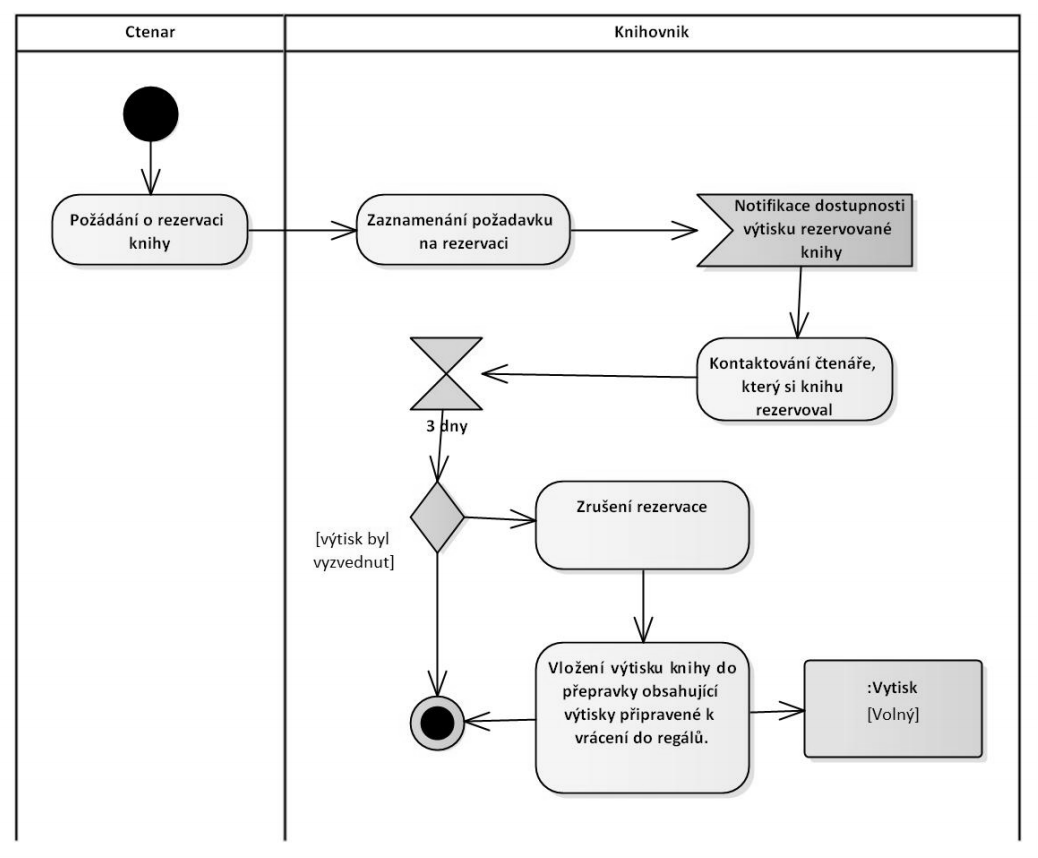
\includegraphics[width=.75\linewidth]{topics/bi-wsi-si-18/images/diagram-aktivit.png}
\caption{Příklad diagramu aktivit}
\end{figure}

\subsection{Chyby}
\begin{itemize}
\item Pro větvení slouží \emph{Rozhodnutí} nebo \emph{Paralelní souběh}.
\item Nemíchat stav objektů s aktivitami.
\end{itemize}
\end{document}
